\documentclass[border=4pt,12pt]{standalone}
% House style for redrawn exam diagrams (diagram-v4: 0.4pt lines, filled -latex arrows, fine dashes; stipple and hatching drawn as real dots/lines (no PDF/SVG patterns, so they render in every browser and at any scale); transparent background). Every figure \input's this.
\usepackage{amsmath,amssymb}
\usepackage{txfonts}
\usepackage{pdfrender,xcolor}
% \halo{text}: label on shading. The shading stops just around each letter's outline (a thin knock-out that follows the
% glyphs, like the papers' typesetting), never a box. Owner: "I don't want a box around the text".
\newcommand{\halo}[1]{\leavevmode\rlap{\pdfrender{TextRenderingMode=2,LineWidth=2.2pt,LineJoinStyle=1,StrokeColor=white,FillColor=white}#1}#1}
\usepackage{tikz,pgfplots}
\pgfplotsset{compat=1.18}
\usetikzlibrary{arrows.meta,calc,angles,quotes,patterns,patterns.meta,intersections,positioning,decorations.markings,shapes.geometric}
% Stipple and hatching are drawn as actual dots / lines clipped to the region (path picture), NOT as pattern fills:
% SVG <pattern> fills vanish or blur when browsers scale the image, so the owner could not see the shading.
% Each dot is a 0.72pt square (keeps SVGs small; reads as a dot at print size). Dots sit on one global staggered grid, so neighbouring regions line up.
\makeatletter
\newdimen\ex@x \newdimen\ex@y \newdimen\ex@xa \newdimen\ex@ya \newdimen\ex@xb \newdimen\ex@yb \newcount\ex@row
\def\exam@stipplecolor{black!75}\def\exam@dotr{0.42pt}\def\exam@dotgap{2.5}
\def\ex@rowdots{\ifdim\ex@x<\ex@xb \pgfpathrectangle{\pgfqpoint{\dimexpr\ex@x-0.36pt\relax}{\dimexpr\ex@y-0.36pt\relax}}{\pgfqpoint{0.72pt}{0.72pt}}\advance\ex@x by \exam@dotgap pt\relax\expandafter\ex@rowdots\fi}
\def\exam@stipple{%
  \pgftransformreset% dots are sized in real points even inside scaled pictures
  \pgfpointanchor{path picture bounding box}{south west}\ex@xa=\pgf@x \ex@ya=\pgf@y
  \pgfpointanchor{path picture bounding box}{north east}\ex@xb=\pgf@x \ex@yb=\pgf@y
  \pgfsetfillcolor{\exam@stipplecolor}\pgfmathsetmacro\ex@h{\exam@dotgap/2}%
  \pgfmathtruncatemacro\ex@r{floor(\ex@ya/\ex@h)-1}\ex@row=\ex@r\relax
  \ex@y=\ex@r\dimexpr\ex@h pt\relax
  \loop\ifdim\ex@y<\ex@yb
    \pgfmathtruncatemacro\ex@c{floor(\ex@xa/\exam@dotgap)-1}\ex@x=\ex@c\dimexpr\exam@dotgap pt\relax
    \ifodd\ex@row \advance\ex@x by \ex@h pt\fi
    \ex@rowdots
    \advance\ex@y by \ex@h pt \advance\ex@row by 1
    \ifnum\numexpr\ex@row-(\ex@row/4)*4\relax=0 \pgfusepath{fill}\fi% flush every 4 rows: bounded TeX memory, few clip copies in the SVG
  \repeat\pgfusepath{fill}}
\newdimen\ex@d
\def\exam@hatch#1{% #1 = 1 for /, -1 for \ ; lines 45 degrees, 3pt apart
  \pgftransformreset
  \pgfpointanchor{path picture bounding box}{south west}\ex@xa=\pgf@x \ex@ya=\pgf@y
  \pgfpointanchor{path picture bounding box}{north east}\ex@xb=\pgf@x \ex@yb=\pgf@y
  \ex@d=\dimexpr\ex@yb-\ex@ya\relax \ex@x=\dimexpr\ex@xa-\ex@d\relax
  \loop\ifdim\ex@x<\ex@xb
    \ifnum#1>0 \pgfpathmoveto{\pgfqpoint{\ex@x}{\ex@ya}}\pgfpathlineto{\pgfqpoint{\dimexpr\ex@x+\ex@d\relax}{\ex@yb}}%
    \else \pgfpathmoveto{\pgfqpoint{\ex@x}{\ex@yb}}\pgfpathlineto{\pgfqpoint{\dimexpr\ex@x+\ex@d\relax}{\ex@ya}}\fi
    \advance\ex@x by 4.24pt
  \repeat
  \pgfsetlinewidth{0.4pt}\pgfsetstrokecolor{black}\pgfusepath{stroke}}
\def\examstipple{\exam@stipple}\def\examhatch{\exam@hatch}\def\examsetstipplecolor#1{\def\exam@stipplecolor{#1}}\def\examsetdotgap#1{\def\exam@dotgap{#1}}
\makeatother
% (legacy pattern kept for old files)
% staggered stipple like the NESA papers' dotted shading
\pgfdeclarepatternformonly{exam stipple}{\pgfpointorigin}{\pgfqpoint{2.2pt}{2.2pt}}{\pgfqpoint{2.2pt}{2.2pt}}{%
  \pgfpathcircle{\pgfqpoint{0.55pt}{0.55pt}}{0.42pt}\pgfpathcircle{\pgfqpoint{1.65pt}{1.65pt}}{0.42pt}\pgfusepath{fill}}
\tikzset{
  every picture/.style={line width=0.6pt, >={Latex[length=2mm,width=1.3mm]}},
  curve/.style={line width=0.6pt},
  open arrow/.style={-{Latex[length=2mm,width=1.3mm]}},  % owner: filled -latex heads everywhere, no open chevrons
  aux/.style={dash pattern=on 2pt off 1.5pt, line width=0.6pt},
  shade/.code={\def\exA{#1}\def\exB{none}\ifx\exA\exB\else\pgfkeysalso{fill=black!18}\fi},
  shade/.default=on,
  shade dots/.style={fill=none, path picture={\examstipple}},
  stipple color/.code={\examsetstipplecolor{#1}},
  stipple gap/.code={\examsetdotgap{#1}},
  shade dense dots/.style={fill=none, stipple gap=1.6, path picture={\examstipple}},
  shade hatch/.style={fill=none, path picture={\examhatch{1}}},
  shade hatch reverse/.style={fill=none, path picture={\examhatch{-1}}},
  shade solid/.style={fill=black},
  pt/.style={circle, fill, inner sep=1.1pt},
  open pt/.style={circle, draw, fill=white, inner sep=1.1pt},
}
\pgfplotsset{
  exam axes/.style={axis lines=middle, axis line style={->}, xlabel={$x$}, ylabel={$y$},
    xlabel style={anchor=west}, ylabel style={anchor=south}, tick label style={font=\small},
    every axis plot/.append style={line width=0.6pt, black}, samples=200, clip=false,
    enlargelimits=false, axis on top},
}

\begin{document}
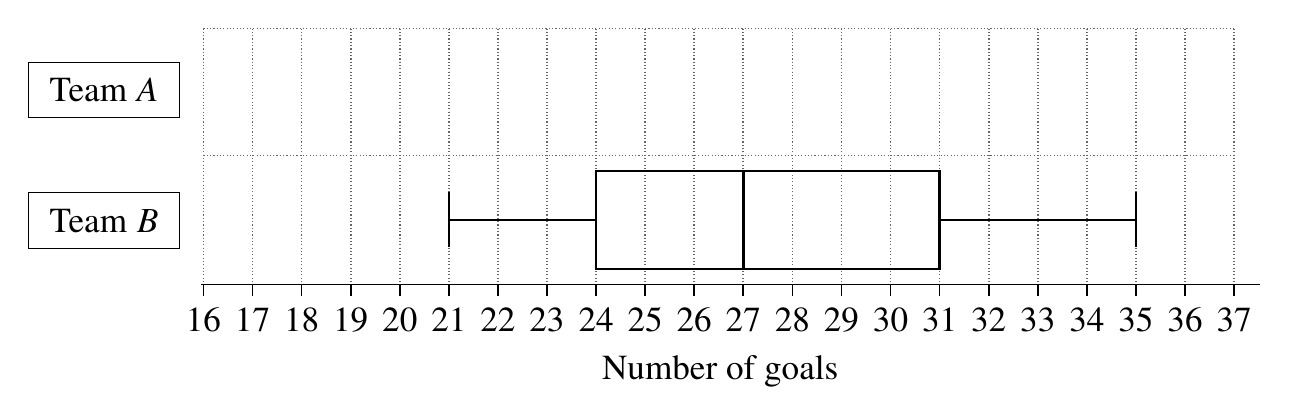
\begin{tikzpicture}[x=0.0127cm,y=-0.0127cm,font=\fontsize{12.7}{15.239999999999998}\selectfont]
\draw[dash pattern=on 0.4pt off 0.8pt,black!60] (220.0,41)--(220.0,296);
\draw[dash pattern=on 0.4pt off 0.8pt,black!60] (269.1,41)--(269.1,296);
\draw[dash pattern=on 0.4pt off 0.8pt,black!60] (318.2,41)--(318.2,296);
\draw[dash pattern=on 0.4pt off 0.8pt,black!60] (367.3,41)--(367.3,296);
\draw[dash pattern=on 0.4pt off 0.8pt,black!60] (416.4,41)--(416.4,296);
\draw[dash pattern=on 0.4pt off 0.8pt,black!60] (465.5,41)--(465.5,296);
\draw[dash pattern=on 0.4pt off 0.8pt,black!60] (514.6,41)--(514.6,296);
\draw[dash pattern=on 0.4pt off 0.8pt,black!60] (563.7,41)--(563.7,296);
\draw[dash pattern=on 0.4pt off 0.8pt,black!60] (612.8,41)--(612.8,296);
\draw[dash pattern=on 0.4pt off 0.8pt,black!60] (661.9,41)--(661.9,296);
\draw[dash pattern=on 0.4pt off 0.8pt,black!60] (711.0,41)--(711.0,296);
\draw[dash pattern=on 0.4pt off 0.8pt,black!60] (760.1,41)--(760.1,296);
\draw[dash pattern=on 0.4pt off 0.8pt,black!60] (809.2,41)--(809.2,296);
\draw[dash pattern=on 0.4pt off 0.8pt,black!60] (858.3,41)--(858.3,296);
\draw[dash pattern=on 0.4pt off 0.8pt,black!60] (907.4,41)--(907.4,296);
\draw[dash pattern=on 0.4pt off 0.8pt,black!60] (956.5,41)--(956.5,296);
\draw[dash pattern=on 0.4pt off 0.8pt,black!60] (1005.6,41)--(1005.6,296);
\draw[dash pattern=on 0.4pt off 0.8pt,black!60] (1054.7,41)--(1054.7,296);
\draw[dash pattern=on 0.4pt off 0.8pt,black!60] (1103.8,41)--(1103.8,296);
\draw[dash pattern=on 0.4pt off 0.8pt,black!60] (1152.9,41)--(1152.9,296);
\draw[dash pattern=on 0.4pt off 0.8pt,black!60] (1202.0,41)--(1202.0,296);
\draw[dash pattern=on 0.4pt off 0.8pt,black!60] (1251.1,41)--(1251.1,296);
\draw[dash pattern=on 0.4pt off 0.8pt,black!60] (220.0,41)--(1251.1,41);
\draw[dash pattern=on 0.4pt off 0.8pt,black!60] (220.0,168)--(1251.1,168);
\draw (218,297)--(1277,297);
\draw (220.0,297)--(220.0,309);
\node[anchor=base,inner sep=0] at (220.0,344) {16};
\draw (269.1,297)--(269.1,309);
\node[anchor=base,inner sep=0] at (269.1,344) {17};
\draw (318.2,297)--(318.2,309);
\node[anchor=base,inner sep=0] at (318.2,344) {18};
\draw (367.3,297)--(367.3,309);
\node[anchor=base,inner sep=0] at (367.3,344) {19};
\draw (416.4,297)--(416.4,309);
\node[anchor=base,inner sep=0] at (416.4,344) {20};
\draw (465.5,297)--(465.5,309);
\node[anchor=base,inner sep=0] at (465.5,344) {21};
\draw (514.6,297)--(514.6,309);
\node[anchor=base,inner sep=0] at (514.6,344) {22};
\draw (563.7,297)--(563.7,309);
\node[anchor=base,inner sep=0] at (563.7,344) {23};
\draw (612.8,297)--(612.8,309);
\node[anchor=base,inner sep=0] at (612.8,344) {24};
\draw (661.9,297)--(661.9,309);
\node[anchor=base,inner sep=0] at (661.9,344) {25};
\draw (711.0,297)--(711.0,309);
\node[anchor=base,inner sep=0] at (711.0,344) {26};
\draw (760.1,297)--(760.1,309);
\node[anchor=base,inner sep=0] at (760.1,344) {27};
\draw (809.2,297)--(809.2,309);
\node[anchor=base,inner sep=0] at (809.2,344) {28};
\draw (858.3,297)--(858.3,309);
\node[anchor=base,inner sep=0] at (858.3,344) {29};
\draw (907.4,297)--(907.4,309);
\node[anchor=base,inner sep=0] at (907.4,344) {30};
\draw (956.5,297)--(956.5,309);
\node[anchor=base,inner sep=0] at (956.5,344) {31};
\draw (1005.6,297)--(1005.6,309);
\node[anchor=base,inner sep=0] at (1005.6,344) {32};
\draw (1054.7,297)--(1054.7,309);
\node[anchor=base,inner sep=0] at (1054.7,344) {33};
\draw (1103.8,297)--(1103.8,309);
\node[anchor=base,inner sep=0] at (1103.8,344) {34};
\draw (1152.9,297)--(1152.9,309);
\node[anchor=base,inner sep=0] at (1152.9,344) {35};
\draw (1202.0,297)--(1202.0,309);
\node[anchor=base,inner sep=0] at (1202.0,344) {36};
\draw (1251.1,297)--(1251.1,309);
\node[anchor=base,inner sep=0] at (1251.1,344) {37};
\node[anchor=base west,inner sep=0] at (618,392) {Number of goals};
\draw (45,75) rectangle (196,130); \node[inner sep=0] at (120.5,102.5) {Team $A$\vphantom{T}};
\draw (45,205) rectangle (196,261); \node[inner sep=0] at (120.5,233.0) {Team $B$\vphantom{T}};
\draw[line width=0.9pt] (612.8,183.5) rectangle (956.5,281.5); \draw[line width=0.9pt] (760.1,183.5)--(760.1,281.5);
\draw[line width=0.9pt] (465.5,232.5)--(612.8,232.5); \draw[line width=0.9pt] (956.5,232.5)--(1152.9,232.5);
\draw[line width=0.9pt] (465.5,205.0)--(465.5,260.0); \draw[line width=0.9pt] (1152.9,205.0)--(1152.9,260.0);\end{tikzpicture}
\end{document}
